% !TeX root = ../../main.tex

\chapter{Background}

\lipsum[1]

\begin{equation}
    E = mc^2
\end{equation}

\lipsum[2]

\section{Celestial Bodies in the Solar System}

\lipsum[3]

\begin{figure}[ht]
	% Figures and tables are centred by default
	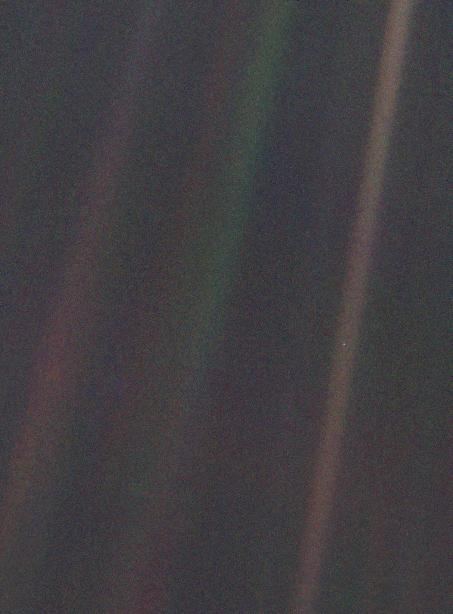
\includegraphics[width=0.6\textwidth]{pale-blue-dot}
	\caption[Pale Blue Dot]{{\bf Pale Blue Dot.} The \emph{Voyager 1} spacecraft took this photograph of planet Earth on February 14, 1990 when she was more than six billion kilometers away from our home.}
\end{figure}

\subsection{Inner Planets}

\lipsum[4]

\begin{table}[ht]
    \begin{tabular}{lcccc}
        \toprule
                & \textbf{Mass} & \textbf{Diameter} & \textbf{Density}  & \textbf{Gravity} \\
                & $10^{24}$ kg  & km                & kg/m$^3$          & m/s$^2$ \\
        \midrule
        Mercury & 0.33          & 4,879             & 5,427             & 3.7 \\
        Venus   & 4.87          & 12,104            & 5,243             & 8.9 \\
        Earth   & 5.97          & 12,756            & 5,514             & 9.8 \\
        Mars    & 0.64          & 6,792             & 3,933             & 3.7 \\
        \bottomrule
    \end{tabular}
    \caption[Comparison of Inner Planets of the Solar System]{{\bf Comparison of Inner Planets of the Solar System.} Lorem ipsum dolor sit amet, consectetur adipiscing elit. Vivamus pellentesque dictum neque, sollicitudin accumsan purus porttitor vitae. Phasellus faucibus enim.}
\end{table}

\lipsum[5]

\begin{figure}[p]
    \caption[Inner Planets of the Solar System]{{\bf Inner Planets of the Solar System}}
    \begin{subfigure}[b]{0.5\textwidth}
        % While figures and tables are centred by default, subfigures and subtables are not
        \centering
        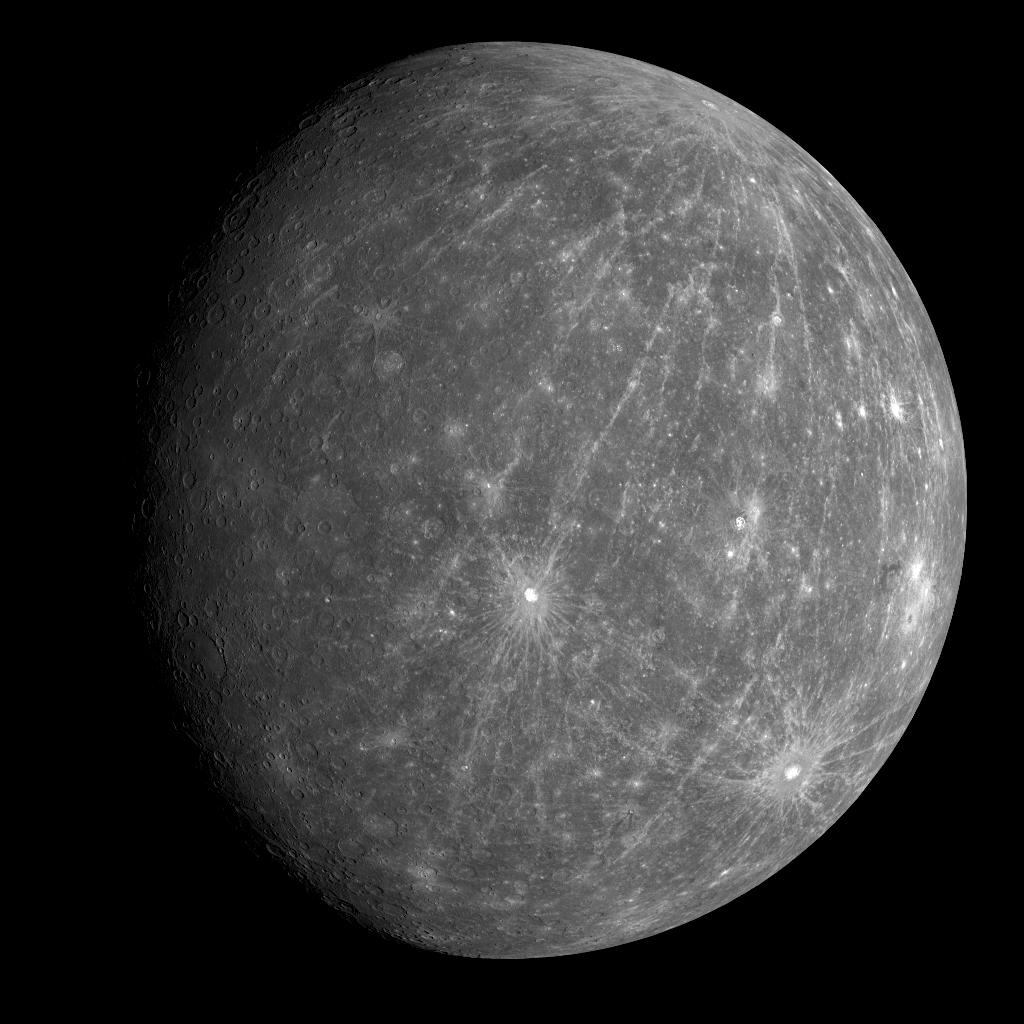
\includegraphics[height=2in]{mercury}
        \caption{Mercury}
    \end{subfigure}%
    \begin{subfigure}[b]{0.5\textwidth}
        \centering
        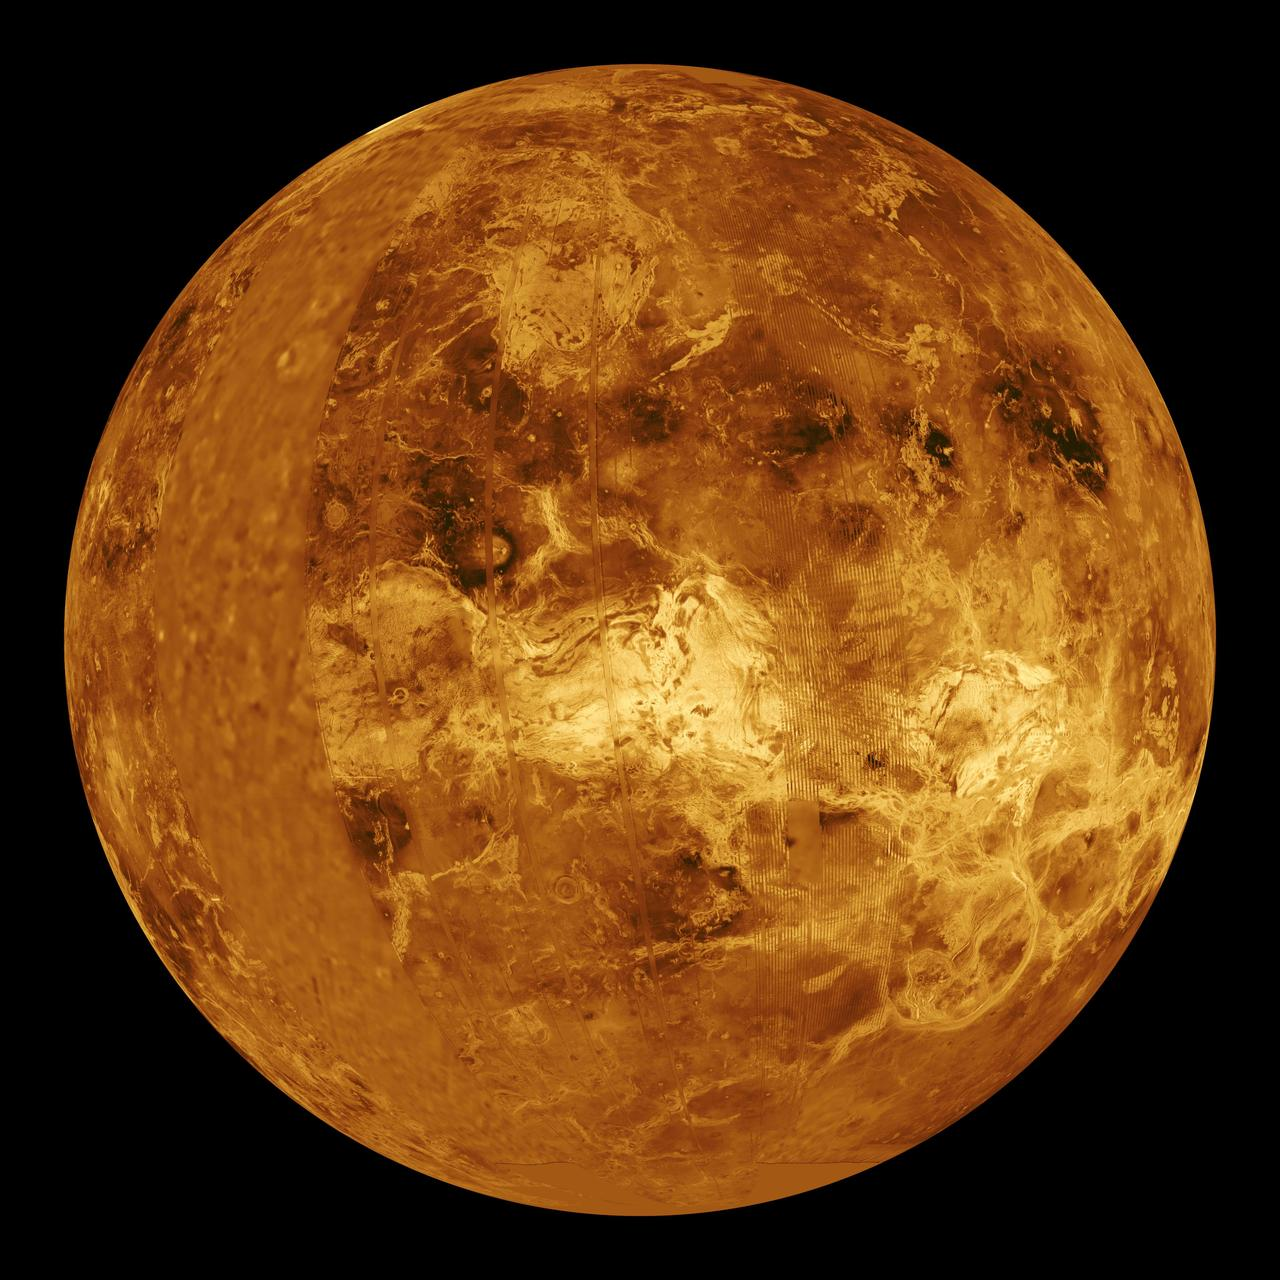
\includegraphics[height=2in]{venus}
        \caption{Venus}
    \end{subfigure}
    % Add space between rows
    \subfigurerow
    \begin{subfigure}[b]{0.5\textwidth}
        \centering
        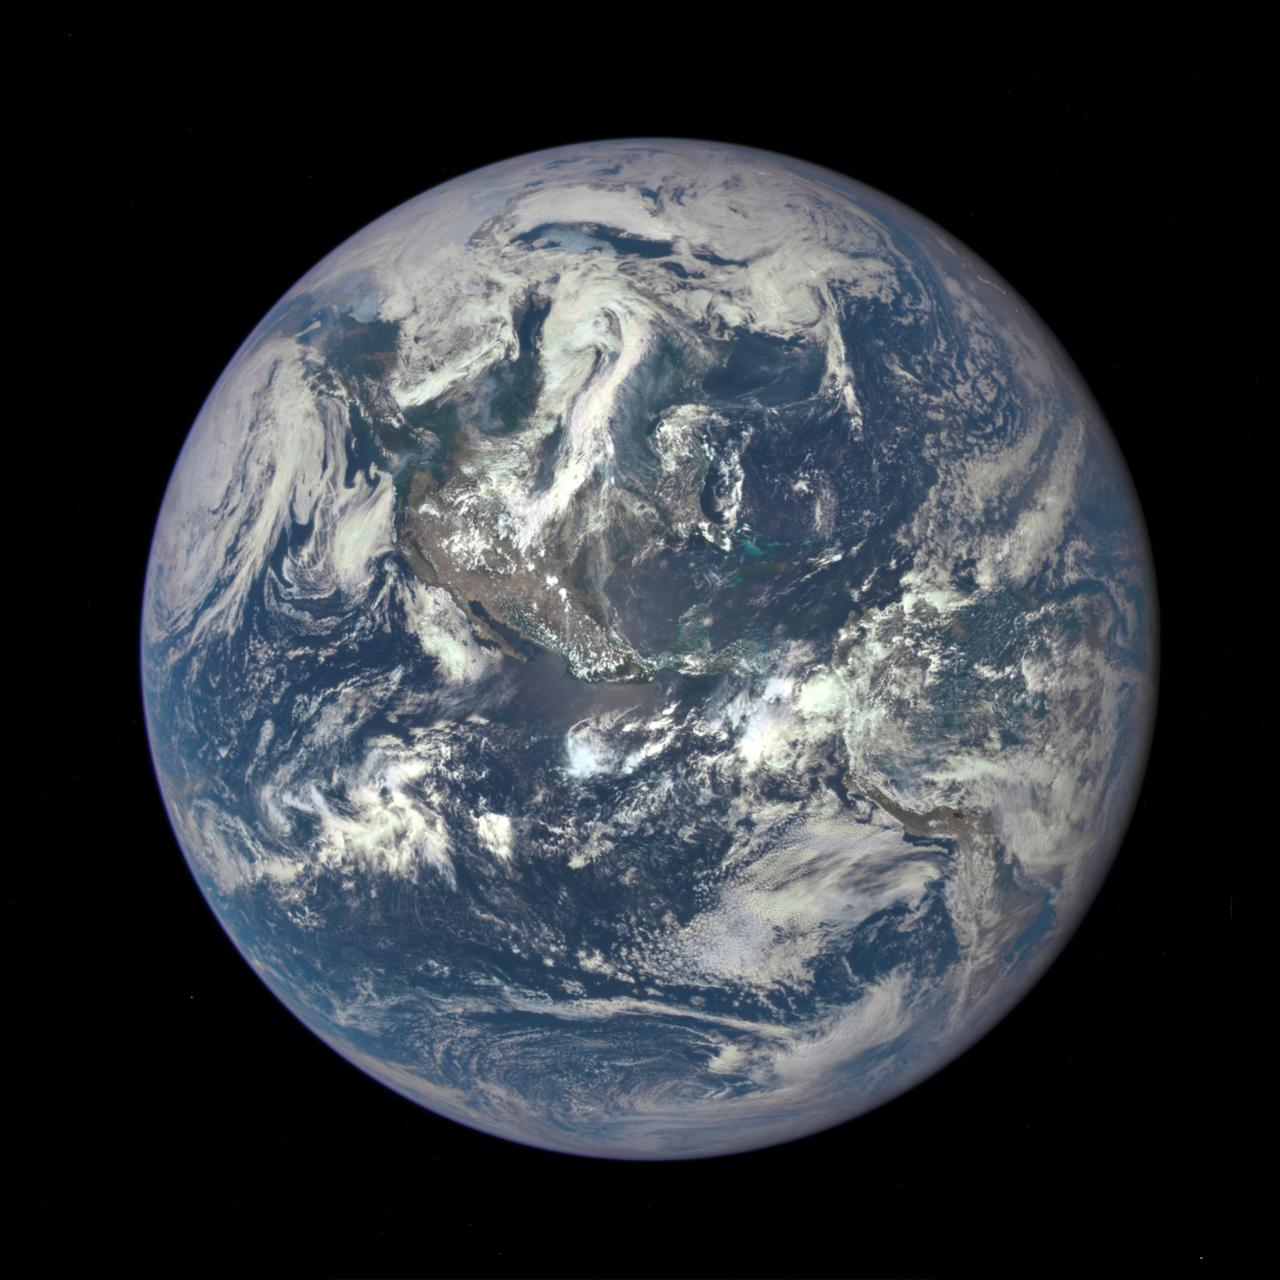
\includegraphics[height=2in]{earth}
        \caption{Earth}
    \end{subfigure}%
    \begin{subfigure}[b]{0.5\textwidth}
        \centering
        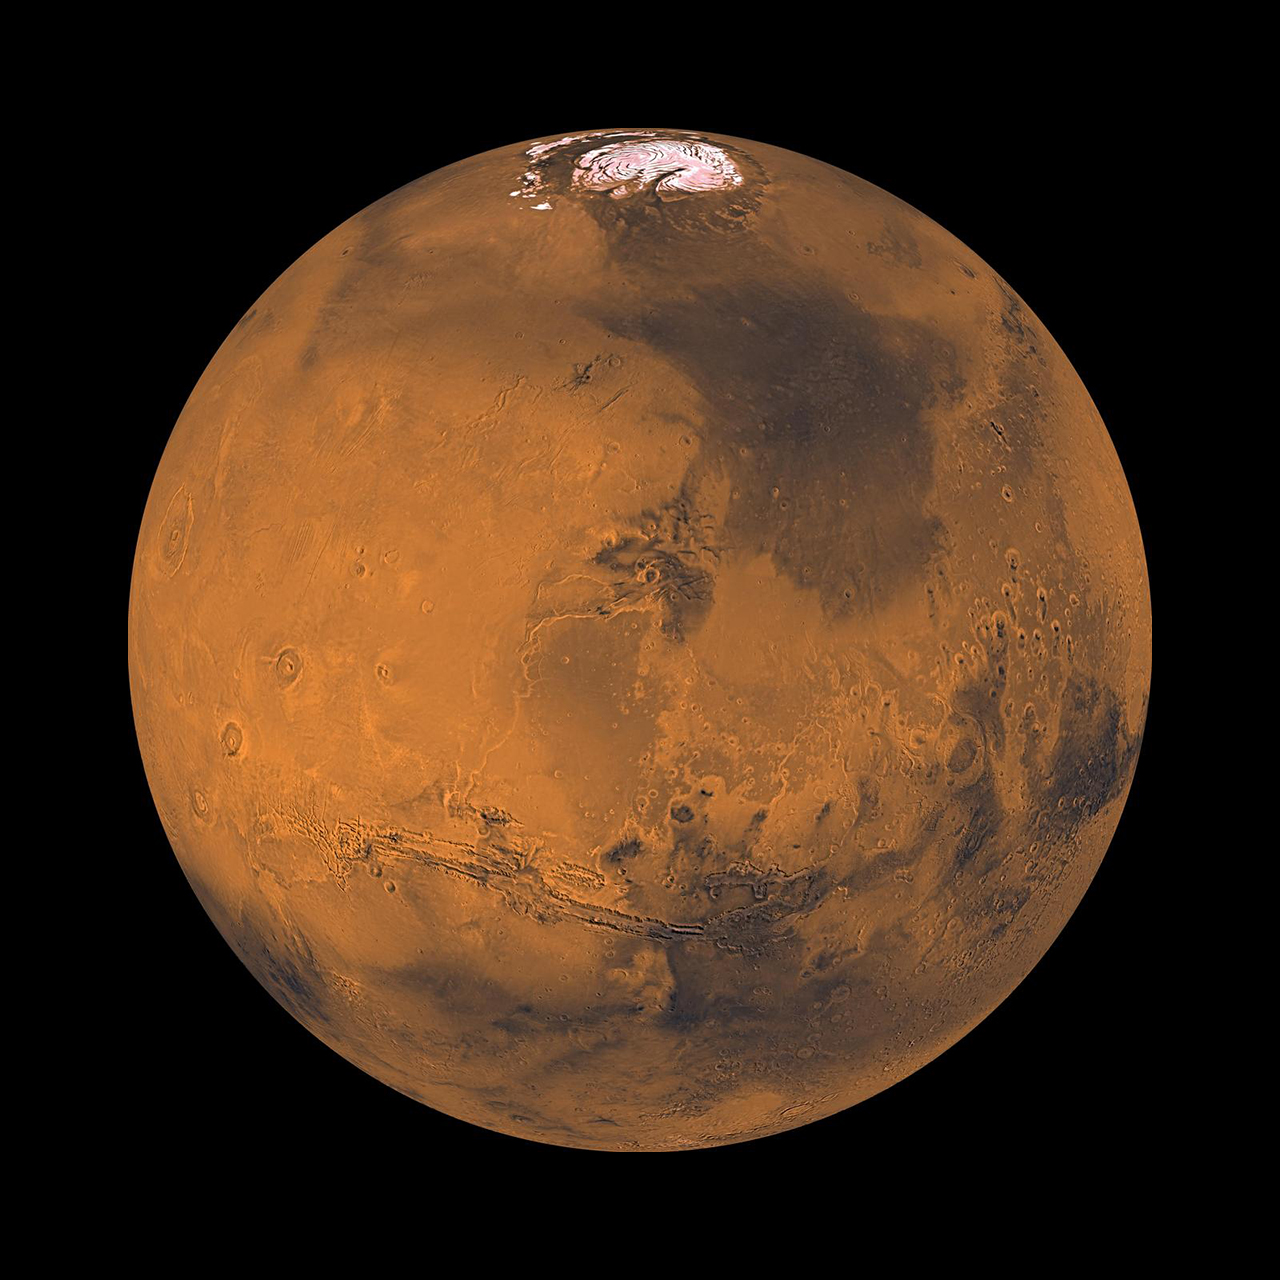
\includegraphics[height=2in]{mars}
        \caption{Mars}
    \end{subfigure}
\end{figure}

\subsection{Asteroid Belt}

\lipsum[6]

\subsection{Outer Planets}

\lipsum[7]

\subsection{Kuiper Belt}

\lipsum[8]

\section{Artificial Objects in Heliocentric Orbits}

\lipsum[9]

\subsection{Tesla Roadster and Starman}

\lipsum[10]

\begin{figure}[ht]
    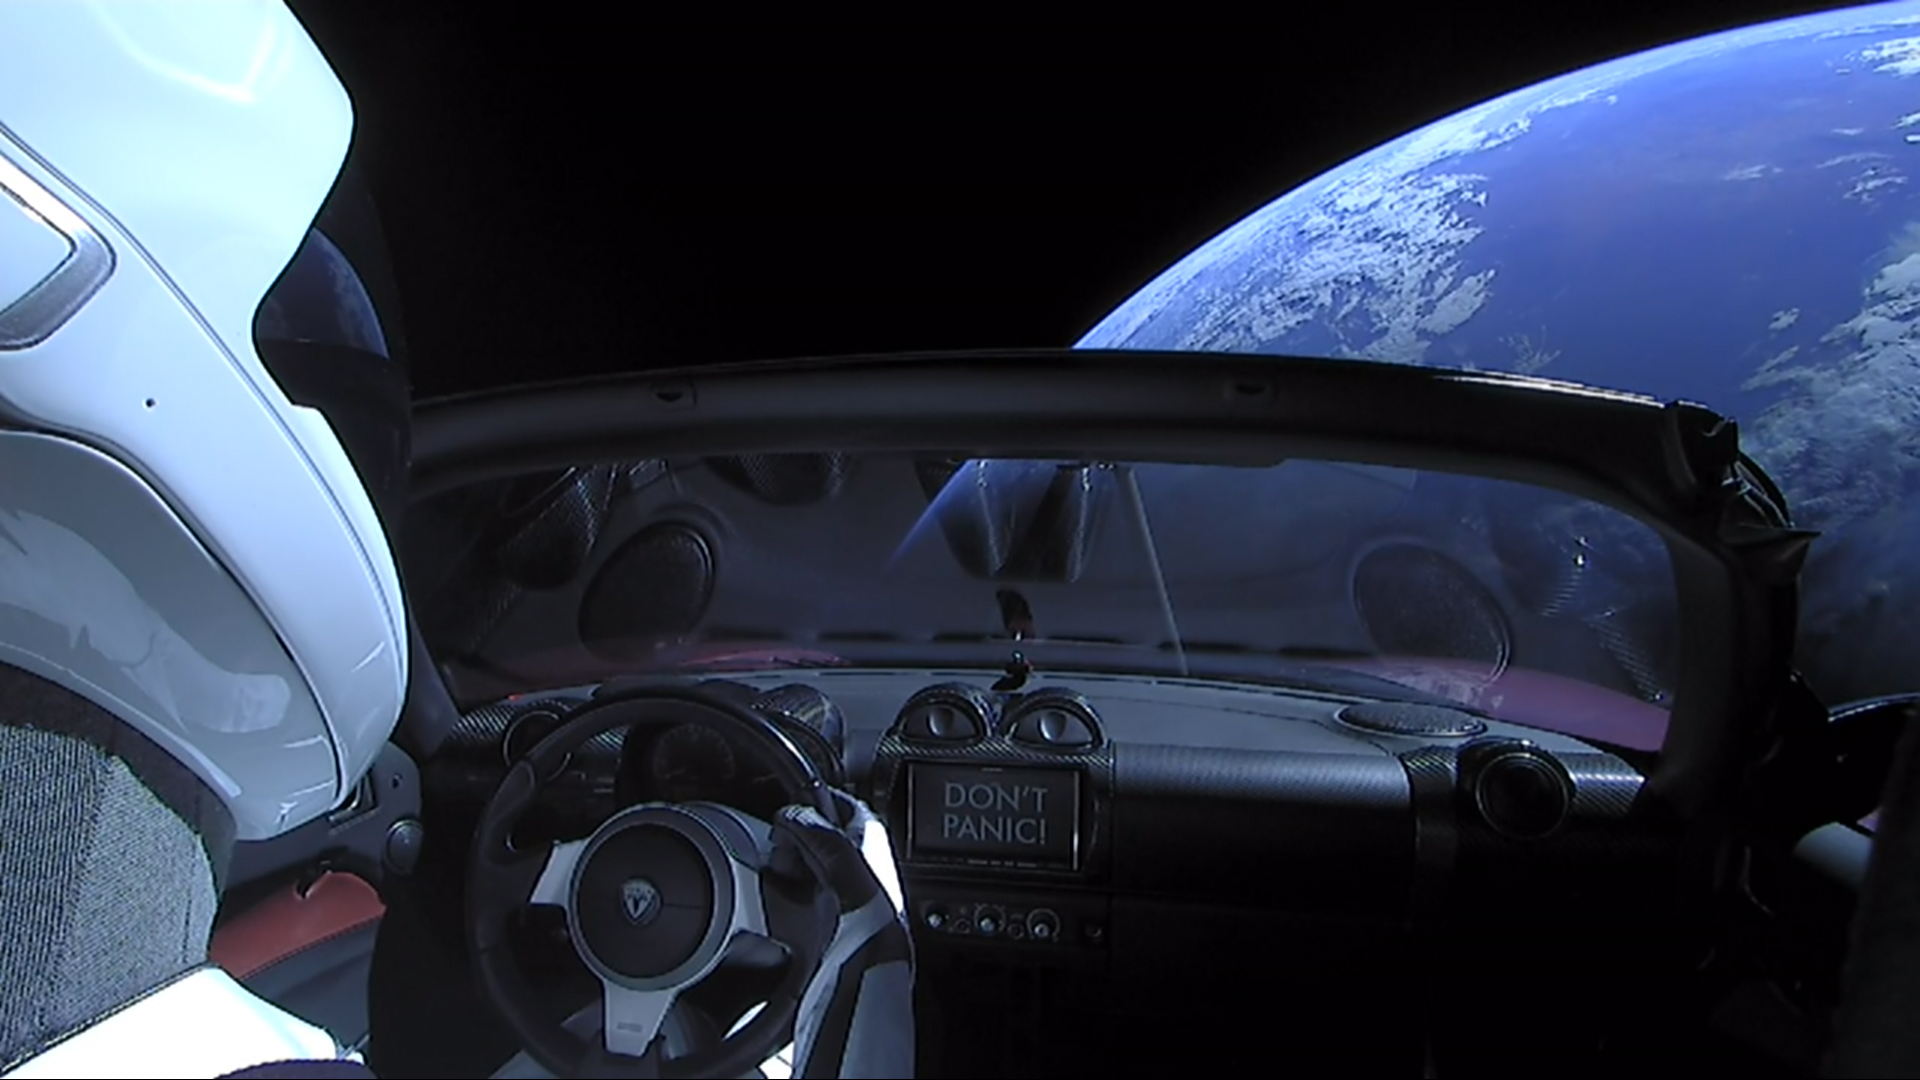
\includegraphics[width=0.8\textwidth]{starman}
    \caption[Don't Panic]{{\bf Don't Panic.} During the maiden flight of SpaceX's Falcon Heavy launch vehicle on February 6, 2018, a Tesla Roadster electric car with the ``Starman'' mannequin in spacesuit is launched into a heliocentric orbit.}
\end{figure}

\lipsum[11]

\begin{equation}
    \Delta v = v_\text{e} \ln \frac{m_0}{m_f}
\end{equation}

\lipsum[12]
